\documentclass{article}
\usepackage[utf8]{inputenc}
\usepackage[polish]{babel}
\usepackage[T1]{fontenc}
\usepackage{graphicx}
\usepackage{amsmath}
\usepackage{tikz}
\usepackage{mathdots}
\usepackage{yhmath}
\usepackage{cancel}
\usepackage{color}
\usepackage{siunitx}
\usepackage{array}
\usepackage{multirow}
\usepackage{amssymb}
\usepackage{gensymb}
\usepackage{tabularx}
\usepackage{booktabs}
\usepackage{multicol}
\usepackage{comment}
\usetikzlibrary{fadings}
\usetikzlibrary{patterns}
\usetikzlibrary{shadows.blur}
\usetikzlibrary{shapes}


\title{ Zagraj w hokeja z ładunkami elektrycznymi \\
\large Dokumentacja}

\author{Kamil Sikora,
Maciej Ładoś,
Michał Bar}
\date{April 2020}

\begin{document}

\maketitle

\newpage
\tableofcontents

\newpage

\section{Opis projektu}
Projekt polega na symulacji gry w hokeja z dodatnio naładowanym krążkiem poruszanym jedynie poprzez wpływ innych ładunków elektrycznych. Gracz sam decyduje o rozmieszczeniu ładunków. Celem gry jest umieszczenie krążka w bramce. Gra kończy się po strzeleniu gola lub dotknięciu przez krążek któregoś z ładunków bądź przeszkód.\\
Projekt zdecydowaliśmy się wykonać w JavaScript

\section{Model fizyczny}
Fizyka w grze jest oparta na prawie Coulomba, którego treść brzmi: Siła wzajemnego oddziaływania dwóch naładowanych cząstek jest wprost proporcjonalna do iloczynu wartości tych ładunków i odwrotnie proporcjonalna do kwadratu odległości między nimi.

$$F=k \frac{q 1 \cdot q 2}{r^{2}}$$
$F$ - siła elektrostatyczna \\
$q1, q2$ - ładunki elektryczne \\
$r$ - odległość \\
$k$ - stała elektrostatyczna w przybliżeniu równa $9 \cdot 10^9 \frac{N \cdot m^2}{C^2}$
\\

\noindent Oba ładunki mają również masę, lecz w świecie cząstek, atomów i cząsteczek chemicznych, możemy całkowicie zaniedbać ich wzajemne oddziaływania grawitacyjne.


\begin{figure}[h]
    \centering
    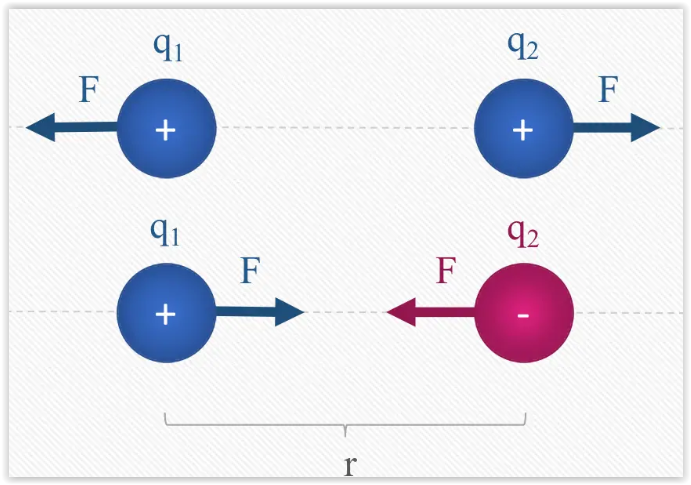
\includegraphics[scale=0.5]{img/Prawo_Coulomba.PNG}

    \caption{Prawo Coulomba- oddziaływanie ładunków}
    \label{fig:Prawo_Coulomba}
\end{figure}

\clearpage

\section{Model symulacyjny}

Nasza symulacja operuje w płaszczyźnie dwuwymiarowej. Każdy obiekt będzie posiadał dwie współrzędne - $x$ i $y$. Odległość między ciałami może być zatem wyznaczona jako odległość punktów na płaszczyźnie.

$$
r=\sqrt{\left(x_{b}-x_{a}\right)^{2}+\left(y_{b}-y_{a}\right)^{2}}
$$

\noindent W celu uproszczenia obliczeń siłę $\vec{F}$ oddziałującą na ładunki rozkładamy na składowe $\vec{F_x}$ oraz $\vec{F_y}$. Zakładamy, że środkiem naszego układu współrzędnych będzie krążek -- pozwoli nam to na skorzystanie z funkcji trygonometrycznych do wyliczenia tych składowych.

\tikzset{every picture/.style={line width=0.75pt}} %set default line width to 0.75pt

\tikzset{every picture/.style={line width=0.75pt}} %set default line width to 0.75pt        

\begin{center}
\begin{tikzpicture}[x=0.75pt,y=0.75pt,yscale=-1,xscale=1]
%uncomment if require: \path (0,261); %set diagram left start at 0, and has height of 261


%Shape: Right Triangle [id:dp36130500270564525] 
\draw   (387,62) -- (521.5,219) -- (387,219) -- cycle ;
%Straight Lines [id:da4371175600607653] 
\draw    (387,62) -- (387,216) ;
\draw [shift={(387,219)}, rotate = 270] [fill={rgb, 255:red, 0; green, 0; blue, 0 }  ][line width=0.08]  [draw opacity=0] (8.93,-4.29) -- (0,0) -- (8.93,4.29) -- cycle    ;
%Straight Lines [id:da010907474739860756] 
\draw  [dash pattern={on 4.5pt off 4.5pt}]  (387,62) -- (519.5,62.42) ;
\draw [shift={(522.5,62.43)}, rotate = 180.18] [fill={rgb, 255:red, 0; green, 0; blue, 0 }  ][line width=0.08]  [draw opacity=0] (8.93,-4.29) -- (0,0) -- (8.93,4.29) -- cycle    ;
%Straight Lines [id:da31420475263437164] 
\draw    (387,62) -- (519.55,216.72) ;
\draw [shift={(521.5,219)}, rotate = 229.41] [fill={rgb, 255:red, 0; green, 0; blue, 0 }  ][line width=0.08]  [draw opacity=0] (8.93,-4.29) -- (0,0) -- (8.93,4.29) -- cycle    ;

% Text Node
\draw (463,115) node [anchor=north west][inner sep=0.75pt]   [align=left] {$\displaystyle r$};
% Text Node
\draw (383,38) node [anchor=north west][inner sep=0.75pt]   [align=left] {$\displaystyle k$};
% Text Node
\draw (523.5,222) node [anchor=north west][inner sep=0.75pt]   [align=left] {$\displaystyle s$};
% Text Node
\draw (448,228) node [anchor=north west][inner sep=0.75pt]   [align=left] {$\displaystyle y$};
% Text Node
\draw (365,132.4) node [anchor=north west][inner sep=0.75pt]    {$x$};
% Text Node
\draw (361,181.4) node [anchor=north west][inner sep=0.75pt]    {$\vec{F}_{y}$};
% Text Node
\draw (493,30.4) node [anchor=north west][inner sep=0.75pt]    {$\vec{F}_{x}$};
% Text Node
\draw (411,65) node [anchor=north west][inner sep=0.75pt]   [align=left] {$\displaystyle \alpha $};
% Text Node
\draw (519,182.4) node [anchor=north west][inner sep=0.75pt]    {$\vec{F}$};

\end{tikzpicture}
\end{center}

\noindent Korzystając z funkcji trygonometrycznych otrzymamy:

$$
\sin \alpha=\frac{\vec{F}_{x}}{r}=\frac{x}{r} \quad \quad \cos \alpha=\frac{\vec{F}_{y}}{r}=\frac{y}{r}
$$

\noindent Przyjmujemy, że wartości ładunków są takie same, więc pomijamy je w obliczeniach. Wyprowadzamy wzory na składowe:

$$
\vec{F}_{x}=\frac{\sin \alpha}{r^{2}} \quad \vec{F}_{y}=\frac{\cos \alpha}{r^{2}}
$$

\noindent Korzystając z II zasady dynamiki Newtona, wyprowadzamy wzór na przyspieszenie ładunku:

$$
F=m \cdot a \Rightarrow a=\frac{F}{m}
$$

\noindent Ostatecznie wzory:

$$
a_{x}=k \cdot \frac{\sin \alpha}{m \cdot r^{2}} \quad a_{y}=k \cdot \frac{\cos \alpha}{m \cdot r^{2}}
$$

\section{Literatura}
\begin{enumerate}
    \item Zbigniew Kąkol, Kamil Kutorasiński. Prawo Coulomba. 
    \item Zbigniew Kąkol. Fizyka. Kraków 2019
    \item David Halliday, Robert Resnick, Jearl Walker. Podstawy fizyki. Tom 3
\end{enumerate}

\end{document}

